\chapter{Knee Joint Design}

The knee joint presented in this thesis is designed to replace the current passive pin knee joint with a spring wrap clutch for the WPI LARRE exoskeleton (see \autoref{sec:larre}).

\TODO{add more in the intro section for the knee joint design}

\section{Design Parameters}

\subsubsection{Follow a specific equation}

\begin{equation}
    r(\theta) mm = 1.078\theta^4 - 11.184\theta^3 + 26.524\theta^2 - 0.825\theta + 263.59
    \label{eq:KneeJointGeometryEquation}
\end{equation}

\subsubsection{Parameter 2}


\section{Mechanical Design}

The orthotic joint design proposed uses a similar idea to how a human knee joint works; a cam mechanism  extends the shank link as it is rotated relative to the thigh link. The joint therefore has two degrees of freedom: rotation around the center of rotation (output shaft of the motor and gearbox) and translation in the direction of the shank. However, since there is only one actuator, the joint is underactuated; this underactuation can be taken advantage of to match a patient's knee trajectory, where the center of mass of the shank extends away from the joint center as the joint bends.

\begin{figure} [ht!]
    \centering
    \missingfigure{Knee Joint Exploded View}
    \caption{Exploded view of the knee joint, with all relevant components labeled}
    \label{fig:KneeJointExplodedView}
\end{figure}

\subsubsection{Torsion Bars}
The center of rotation of the joint is designed to match the axis of rotation of the actuator. The output of this actuator \fix{Add reference to actuator decision section} is directly connected to the torsion bar using M5 shoulder bolts. Each bolt is designed to support 3 bearings: 2 on the motor side and 1 on the patient side. The reduced count on the patient side allows for the torsion bar to be partially recessed in the shank link to reduce the distance between the center of mass between the patient and the joint. The 6 bearings are still able to support the forces necessary throughout a walking gait cycle (see \autoref{sec:BearingsAndCalcs}). 

\subsubsection{Shank Links}
The 2 shank links attach to the lower part of the exoskeleton, and are responsible for taking the rotational energy created by the motor and partially changing it to translational energy to help linearly extend the shank. The bearings connected to the torsion bars ride in a guide built into the shank link. This guide is slightly larger than the bearing diameter (\(~0.3mm\)) to prevent rubbing without creating much of a backlash (\(0.39^\circ\) backlash, see calculation on \autoref{eq:ShankLinkBacklash}).

\begin{equation}
    Backlash = atan(\frac{\frac{0.3mm}{2}}{22mm}) = 0.39^\circ
    \label{eq:ShankLinkBacklash}
\end{equation}

The surface of the guide must be smooth and parallel to the axis of the bearings to avoid damaging them. Depending on the material and manufacturing method chosen, the surface may require additional machining to ensure it can match these requirements. The length of the guide must be larger than the distance between the centers of the two shoulder bolts plus the maximum distance of linear extension by the knee (\autoref{eq:ExtensionGuideLength}). For this prototype, this length was \(78mm\).

\begin{equation}
    GuideLength \geq TorsionBarC2C + MaxKneeExtension = 44mm + 34mm = 78mm
    \label{eq:ExtensionGuideLength}
\end{equation}

The shank link is also responsible to connect to the lower part of the exoskeleton. Just like the thigh link, this is done through the universal exoskeleton connector developed throughout the WPI LARRE project \cite{SpringWrapClutchKnee}.

The connection between the thigh link and the shank link is very important, as it adds torsional stability and overall rigidness to the entire joint. It was therefore imperative during the design process to create wide surface contact between the thigh and shank links. To reduce the energy lost to friction between these plates, 3.2mm thick Delrin\textsuperscript{\textregistered} slides were laser cut and attached to the shank link. 

Similarly to the torsion bar, the shank link also uses 2 shoulder bolts to clamp the two shank links on the thigh link as well as to give the bearings that ride on the knee path guide a precise surface to mount to. To maintain a consistent clamping force, lock nuts are used since they do not easily back out with movement and vibration. 

\subsubsection{Thigh Link}

\begin{figure}
    \centering
    \missingfigure[]{Add cross section of the joint}
    \caption{A cross section of the knee joint in a \(0^\circ\) position}
    \label{fig:KneeJointCrossSection}
\end{figure}

The thigh link acts as the main mounting point for most things, as well as contains the knee path guide. Just like the shank link, the thigh link has the universal exoskeleton connector used throughout the WPI LARRE project. The motor bracket is connected to the thigh link at two locations using \(20mm\diameter x 50mm\) spacers. These spacers must be strong and stiff, as they transmit the torque between the thigh and shank connector in high load situations. A potentiometer is also mounted inside the thigh link to measure the current angle of the joint, as shown in \autoref{fig:KneeJointCrossSection}. The wire connecting to it is routed through a slot in the thigh link to avoid any interference with the moving shank links. This wire comes out the top and is connected to the main controller of the exoskeleton.

\subsubsection{Knee Path Guide}
The knee path guide is built into the thigh link as a slot. The geometry is calculated using several point measurements connected in SolidWorks with a spline. Each point is split by \TODO{Verify this number}{15 degrees}, and calculated from a pre-determined equation. This equation can be measured from a patient knee (see \autoref{sec:KneeParams}), but throughout the design and testing of this knee joint, \autoref{eq:KneeJointGeometryEquation} from \cite{KinDynKneeJoint} is used. \autoref{fig:CenterPlateGeometry} shows the equation above overlayed on the thigh link.

\begin{figure}[ht!]
    \centering
    \missingfigure{Make a picture of the thigh link with relationship highlighted}
    \caption{The thigh link contains the geometry which the bearings ride on to mimic the tibiofemoral relationship}
    \label{fig:CenterPlateGeometry}
\end{figure}

The joint is designed to be easily adaptable between patients. Therefore, the only customized part in the entire system is the thigh link which holds the knee path guide. All other parts remain the same to decrease cost and improve repairability.

\subsubsection{Torque Requirements \& Actuator Selection}

\begin{figure}[ht!]
    \centering
    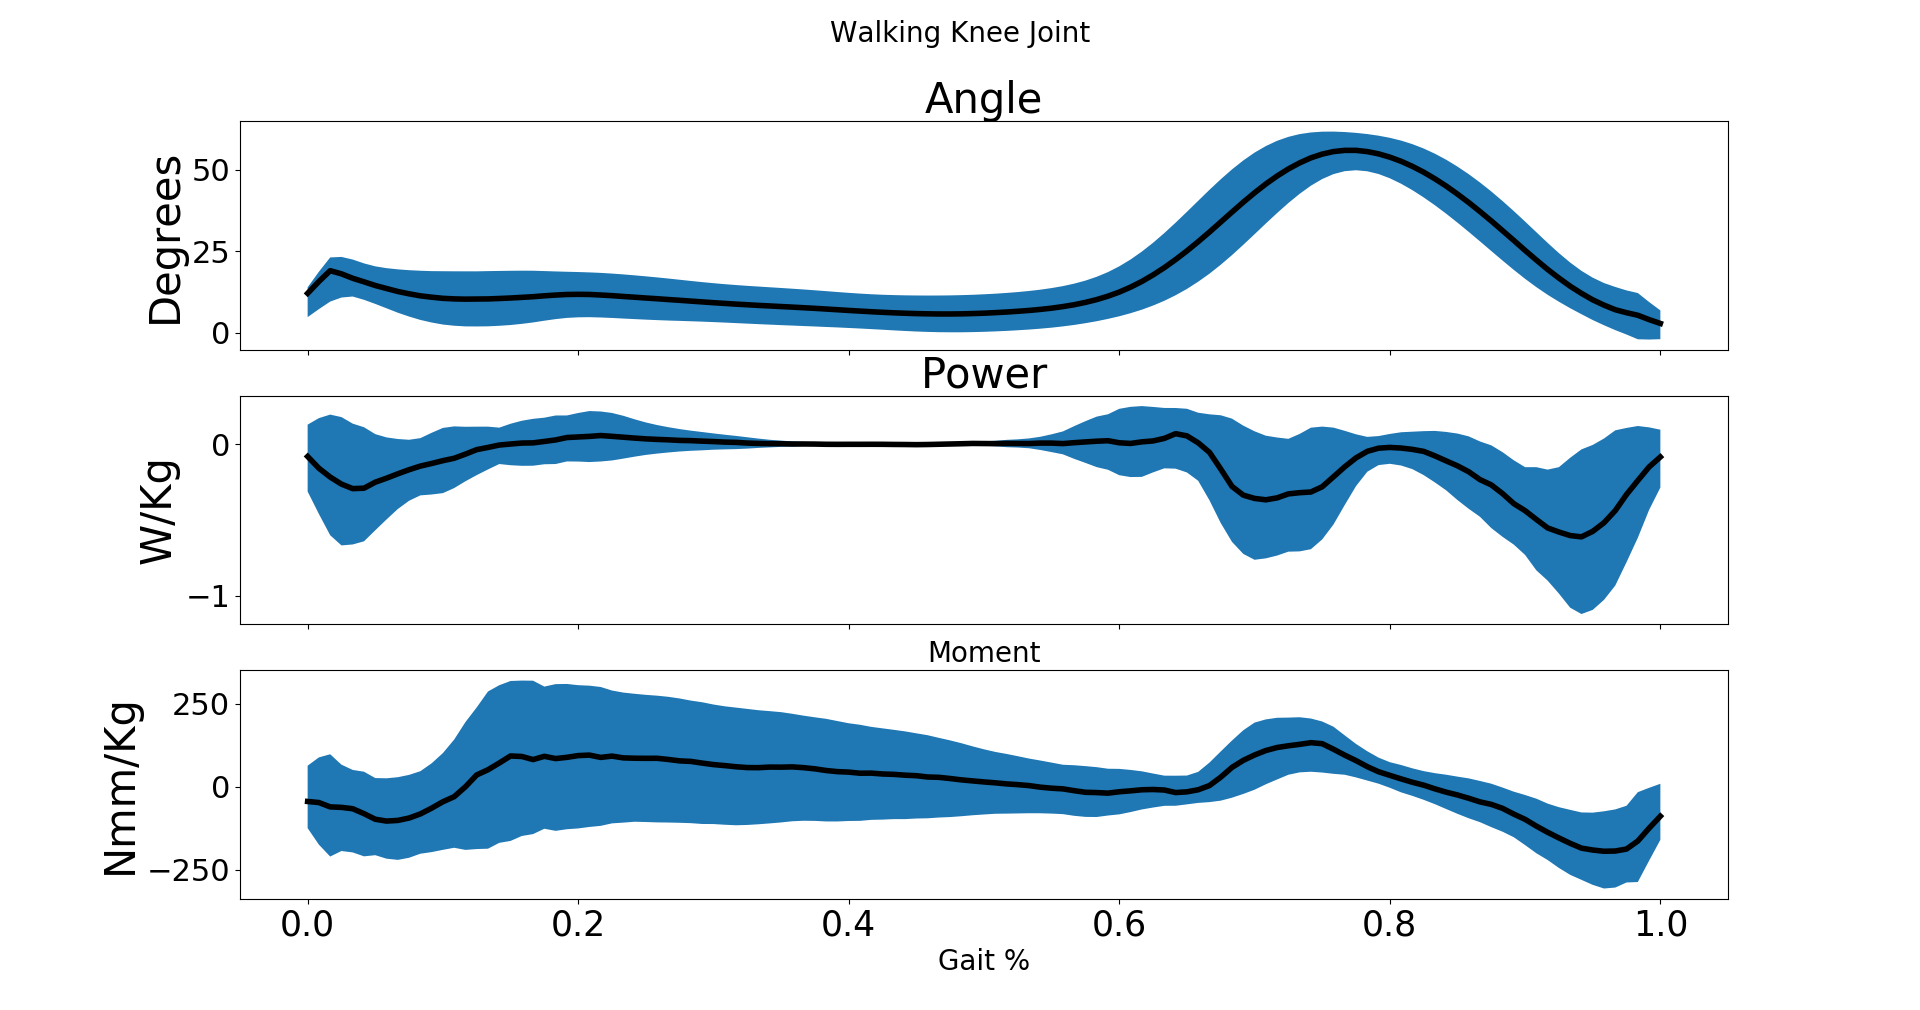
\includegraphics[width=\linewidth]{Figures/Design/WalkingPowerCurveKnee.png}
    \caption{Joint kinematics and dynamics during a walking gait cycle \cite{SpringWrapClutchKnee}}
    \label{fig:WalkingPowerCurve}
\end{figure}

\begin{figure}[ht!]
    \centering
    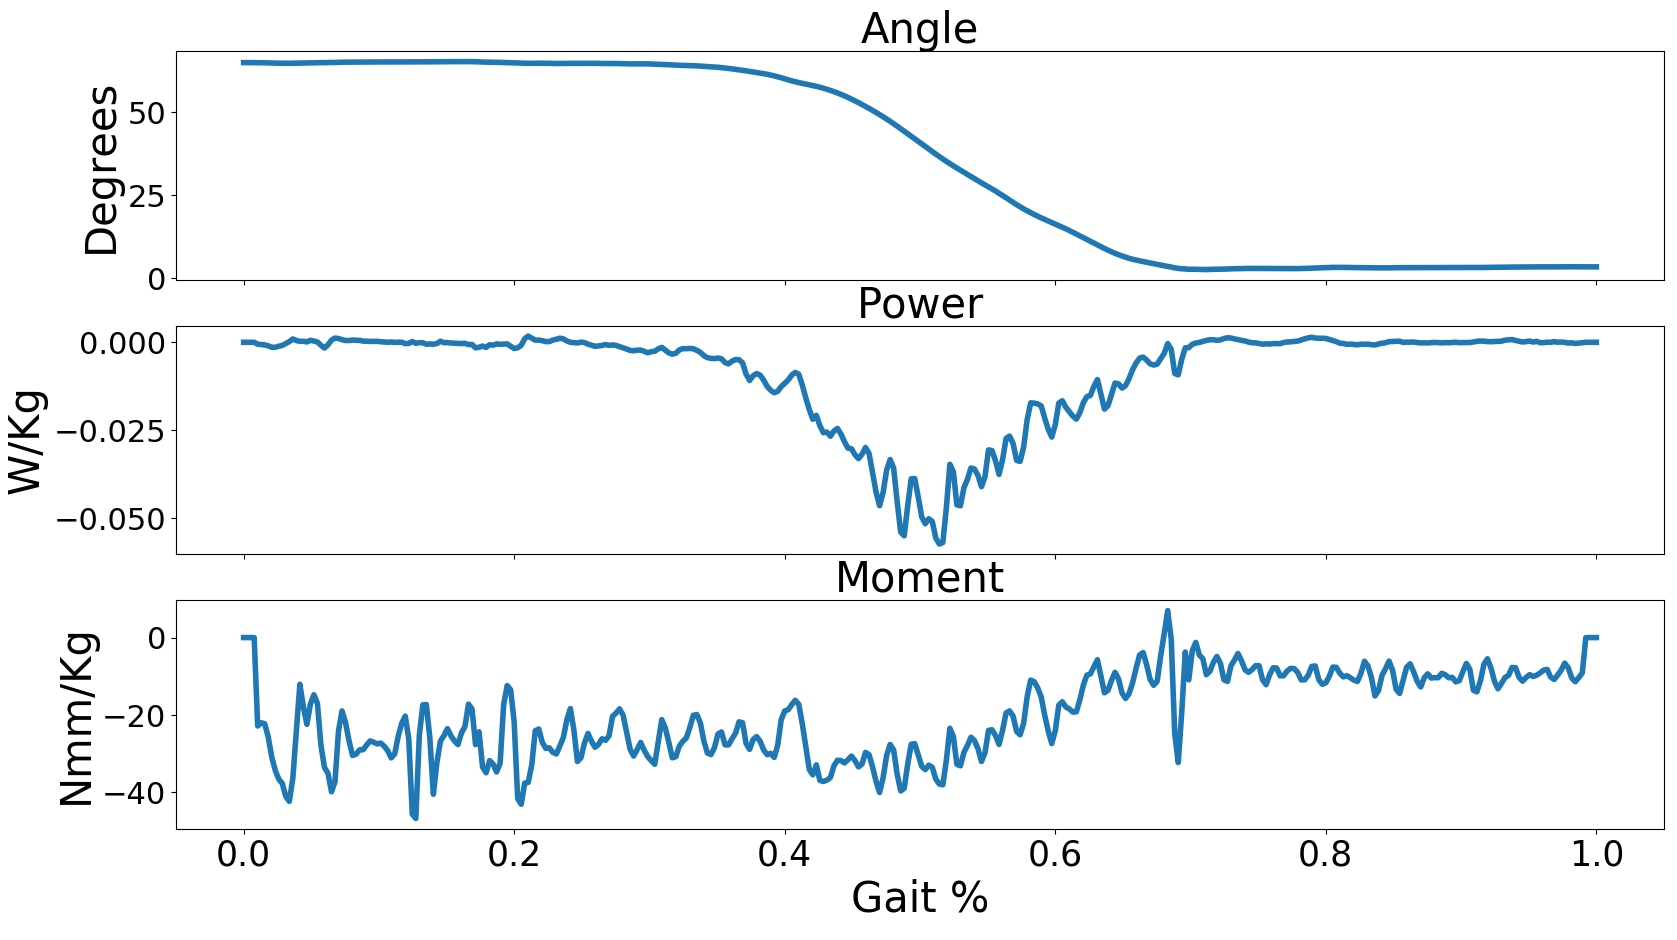
\includegraphics[width=\linewidth]{Figures/Design/SitStandPowerCurveKnee.png}
    \caption{Joint kinematics and dynamics during a sit/stand gait cycle \cite{SpringWrapClutchKnee}}
    \label{fig:SitStandPowerCurve}
\end{figure}

The knee joint has two rehabilitation requirements to fulfill: walking gaits and sit/stand gaits. Prior research has shown that walking gaits require roughly up to \(0.65 \frac{W}{kg}\) and \(0.25\frac{Nm}{kg}\), (see \autoref{fig:WalkingPowerCurve}), while a sit/stand gait requires roughly up to \(0.5 \frac{W}{kg}\) and \(0.04 \frac{Nm}{kg}\). Therefore, the chosen maximum parameters for this knee joint with a \(100 kg\) weight specification is \(65 W\) and \(25 Nm\). \footnote{Peak power reported by the motion capture data is higher, but these parameters were chosen after noise is filtered out. The data is recorded from a normal walking gait of a healthy person.} Speed requirements are roughly \(12^\circ/sec\) for walking gaits and \(15^\circ/sec\) for sit/stand gaits.

The Maxon EC90 was chosen, with a peak power output of \(90W\) and a max continuous torque of \(0.560 Nm\) at \(2510 rpm\) (see \autoref{apx:EC90Datasheet}). To match the speed and torque requirements, a \(100:1\) gearbox ratio is needed. Due to its high reduction to size ratio, a strain wave gearbox from {Harmonic Drives\texttrademark} was chosen.\footnote{The gearbox used is proprietary, and no datasheet is available} Estimated efficiency of this gearbox is roughly \(\epsilon = 90\%\).

\begin{table}
    \centering
    \begin{tabular}{||c|c|c||}
        \hline
        Input (Motor) Power & \(P_{input}\) & \(90 Watts\) \\
        \hline
        Input (Motor) Torque @ Nominal & \(\tau_{input}\) & \(0.560 Nm\) \\
        \hline
        Input (Motor) Speed @ Nominal & \(\omega_{input}\) & \(2510 rpm\) \\
        \hline
        Input (Motor) Stall Torque & \(\tau_{in\_stall}\) & \(7.480 Nm\) \\
        \hline \hline
        Gearbox Ration & \(\frac{n_1}{n_2}\) & \(100:1\) \\
        \hline \hline
        Output Power & \(P_{output}\) & \(81 Watts\) \\
        \hline
        Output Torque @ Nominal & \(\tau_{input}\) & \(50.4 Nm\) \\
        \hline
        Output Speed @ Nominal & \(\omega_{input}\) & \(15^\circ/sec\) \\
        \hline
        Output Stall Torque & \(\tau_{out\_stall}\) & \(673.2 Nm\) \\
        \hline
    \end{tabular}
    \caption{Motor/gearbox specifications and output power specifications of the proposed joint. See \autoref{apx:JointPowerTorqueSpeedCalcs} for all equations and calculations used.}
    \label{table:MotorGearboxSpecs}
\end{table}

The output power of the joint is \(81 W\), with a nominal torque of \(50.4 Nm\) at \(15^\circ/sec\). Power, torque, and speed specifications of the joint theoretically exceed the requirements. Physical testing is needed, however, to ensure that these numbers are accurate and sufficient for a rehabilitation exoskeleton.
 
\subsubsection{Potentiometer and Rotary Encoder}
A potentiometer was embedded into the knee design to act as an absolute rotary encoder to measure the current angle of the joint. It's purpose is twofold: to provide for an absolute angle at any given time and to provide for rough rotary encoding when a the motor (for passive experimentation). As mentioned above, the integration needed to protect the sensitive connection points. The potentiometer chosen was the Vishay PRV6, with \(200^\circ\) of travel, a linear resistance, and \(\pm 1\%\) tolerance, which equates to a sensored tolerance of \(\pm 2^\circ\). 

The motor used also has 3 hall sensors used for pinpointing the position of the rotor versus the stator. Since the motor has a 12 poles and 3 sensors (totaling 36 pulses per revolution) as well as a 100:1 reduction through the gearbox, the hall effect sensors can be used to create an effective 3600 pulses per revolution encoder. When used in conjunction with the absolute encoder, the encoded angle can be very precise.

% \subsubsection{Motor Analog} 
% \TODO{change the name of this}
% \TODO[inline]{Talk about motor/gearbox analog}

\section{Manufacturing, Materials, \& Parts}
Throughout the design, manufacturability and easy assembly was a focus. The entire system is held together with 4 M5 shoulder bots with 6mm diameter shoulders to be used as an accurate bearing surface.

\subsubsection{Bearings}
\label{sec:BearingsAndCalcs}
All 10 bearings used in the design are the same (for simplicity and reduction of cost): 19mm outside diameter x 6mm inside diameter x 6mm thick double shielded ball bearings (Model 626ZZ). Each is rated for \(2.6kN\) dynamic load and \(1.05kN\) static load. Before selecting these bearings, two calculations were required to ensure these bearings could support the forces required.

The first is the requirement of the torsion bar. 

The second force requirement for these bearings were in the knee path cam

\section{Testing \& Results}

\subsection{Material Analysis}

\subsection{Simulation Motion Analysis}

\subsection{Real-world Motion Analysis}
